\documentclass{IEEEtran}
\usepackage{mathtools}
\usepackage{graphicx}
\usepackage{amssymb}
\usepackage{amsmath}
\usepackage{pythonhighlight}
\usepackage[utf8]{inputenc}
\usepackage{fancyhdr}
\usepackage{pythonhighlight}
\usepackage{changepage}
\usepackage{slashbox}
\usepackage{floatrow}
\usepackage{listings}
\usepackage{derivative}
\usepackage[hidelinks]{hyperref}
\usepackage{fontawesome}
\usepackage{caption}
\usepackage{subcaption}
\usepackage[sorting=none,style=ieee]{biblatex}
\usepackage{cleveref}
\usepackage{algorithm}
\usepackage{algpseudocode}
\usepackage{physics}
\usepackage{lipsum}
\usepackage{titlesec}
\usepackage{diagbox}
\usepackage{makecell}
\usepackage{multicol}
\usepackage{titling}
\predate{}
\postdate{}
\date{}

\addbibresource{report.bib}
\title{Analysis of TransUNet: Hybrid CNN-Transformer}
\author{Kutay Ugurlu}

\begin{document}
\maketitle
\nopagebreak
\onecolumn{
\tableofcontents
\listoffigures
\listoftables
}
\twocolumn
\maketitle
\begin{abstract}
    Medical image segmentation is a crucial part of developing healthcare systems, not only in imaging in the conventional sense but also in electrical source imaging of the brain and heart \cite{gonzalez2020ecgi}. So far, U-Net\cite[text]{ronneberger2015u} has become ubiquitous in medical image segmentation tasks due to its recognized performance. However, the intrinsic features of convolutional neural networks(CNNs) that extract the local features of the spatial region in the image, the architecture exhibits some limitations in finding the long-range patterns. On the other hand, transformers, that were developed for sequence-to-sequence predictions, can recognize the global patterns via the utilization of attention mechanism \cite{vaswani2017attention}. Chen, \textit{et al.}, propose a hybrid CNN-Transformer network called TransUNet in their study  \cite{chen2021transunet} to tackle the problem of medical image segmentation exploiting both local and global dependencies in the images.
    In this project, the aforesaid study is analyzed and a series of experiments is conducted whose results are available online at the forked repository: \href{https://github.com/kutay-ugurlu/TransUNet_Analysis}{https://github.com/kutay-ugurlu/TransUNet\_Analysis}. 
\end{abstract}
\section{Introduction}

Image segmentation is a semantic segmentation task where each of the pixels (or voxels) is assigned a class corresponding to the object that they represent. Medical image segmentation has been of particular interest to researchers for diagnosis, treatment, and even prognosis, in different fields. Given the small size of medical datasets available, the segmentation is a challenging task \cite{ren2019brain}. Furthermore, especially in human imaging, the segmentation boundaries need to be precise to make reliable decisions on the data. Hence, a model has to be trained to separate the organ and physiological boundaries successfully with a high spatial resolution, as in \Cref{fig:brainseg}, while also having the capability to generalize to other data distributions it may be fed. 

\begin{figure}[h]
    \centering
    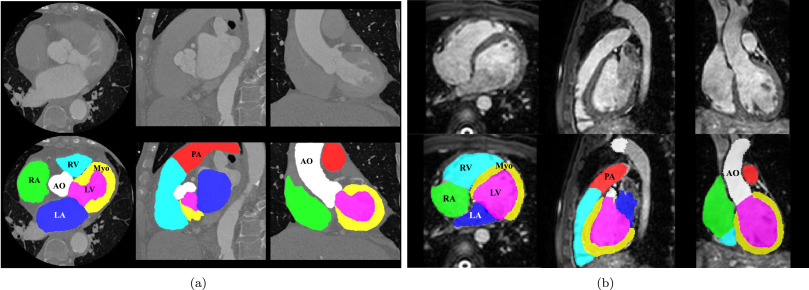
\includegraphics[width=\textwidth]{img/heartseg1.jpg}
    \caption{Whole Heart Segmentation \cite{ZHUANG2019101537}}\label{fig:heartseg}
    \end{figure}

\begin{figure}[h]
    \centering
    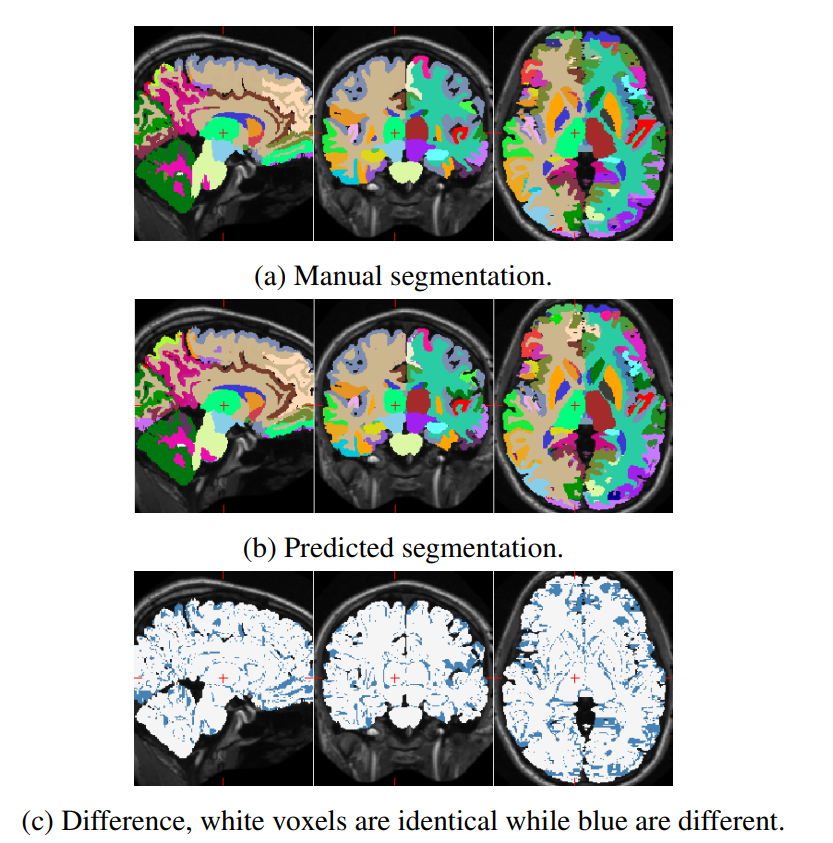
\includegraphics[width=\textwidth]{img/brainseg.png}
    \caption{Whole Brain Segmentation \cite{de2015deep}}\label{fig:brainseg}
    \end{figure}


To improve both the local and global pattern recognition capability, the authors of \cite{chen2021transunet} propose a hybrid network whose components are going to be analyzed individually in the following sections. 

\section{Theory}

\subsection{U-Net}
U-Net is a convolutional neural network that utilizes certain modifications compared to its predecessors. 

\begin{figure}[h]
\centering
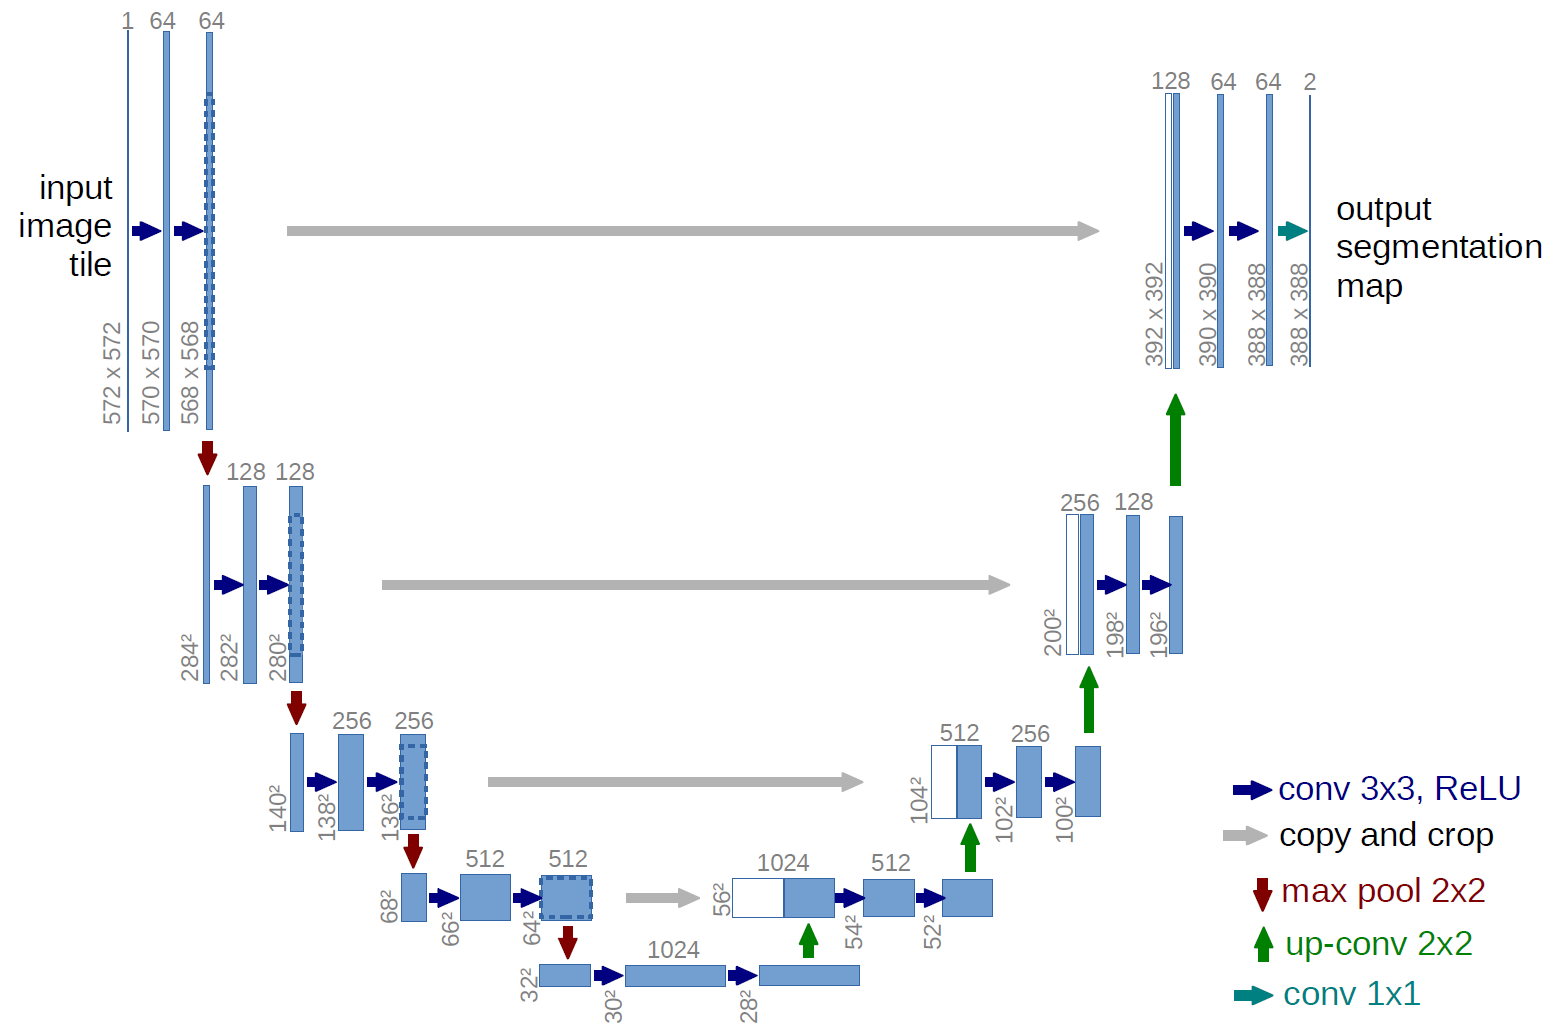
\includegraphics[width=\textwidth]{img/u-net-architecture.png}
\caption{A generic U-Net Architecture}\label{fig:unet}
\end{figure}

\vfill\null\newpage
The U-Net Architecture has the following properties that enable it to perform well in assigning classes to each pixel: 

\begin{itemize}
    \item Multilevel Decomposition: For shrinking image sizes,  it utilizes the same size of convolutional kernels. In other words, for convolution, it employs different Fourier transform sizes to match different images size allowing it to decompose the image in multiple different spatial frequencies. 
    \item Residual Learning: The skip connections created between input and output, along with the encoded features in the encoder pathway and the decoded image from latent features, helps the model to learn also from the features encoded before the latent representation and speeds up the training and provide a good convergence rate, avoiding the vanishing gradient problem, borrowing the idea that was proposed for ResNet in \cite{he2016deep}. 
\end{itemize}

Thanks to the multichannel filtering feature of the CNNs, U-Net outputs usually more than one channel corresponding to the foreground (with the segmentation class counts)
and the background. Using a proper cost function, such as mean squared error and an appropriate optimizer, the model learns the function that maps the pixels to the classification labels.  

\subsection{Attention}

Attention was first proposed for sequence-to-sequence tasks, such as machine translation. Since it is developed for natural language processing, its mechanism is illustrated using "words". In tasks, such as machine translation, the input's contextual location or the other words in the sentence might have a huge effect on the input, as in \Cref{fig:attention}, where the word "it" refers to two different words although it is in the same location in the sentence. However, what it refers to is changed by global dependency. In other words, the word at the very end of the sentence had an impact on the word itself. Hence, contextual similarity should also be learned when training sequence-to-sequence models. 
\begin{figure}[h]
\centering
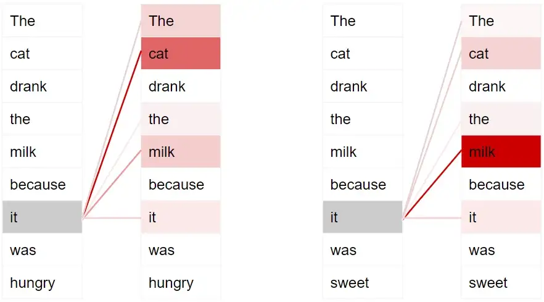
\includegraphics[width=\textwidth]{img/attention.png}
\caption{Words' contextual relation in the sentence \cite{doshi_2021}}\label{fig:attention}
\end{figure}

\vfill\null\newpage
To learn such a relationship, the following mechanism is proposed: 
\begin{figure}[h]
\centering
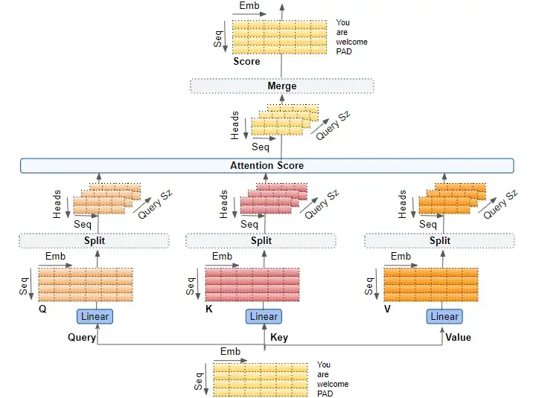
\includegraphics[width=0.8\textwidth]{img/attmech.png}
\caption{MultiHead Self Attention Mechanism}\label{fig:attmech}
\end{figure}

In \Cref{fig:attmech}, the sentence "You are welcome." is padded by one word, and the words are transformed into vectors, or embedding, via an embedding network such as Word2Vec \cite{mikolov2013efficient}. In this example, the embedding size is 6. Then, the embedding is transformed by some trainable linear transformations, or matrices $W_Q, W_K, W_V$, to three different spaces, \textbf{Query}, \textbf{Key} and \textbf{Value}. Following this operation, the projections are split into different attention heads, and the relationship weights are calculated using $\sigma(QK^T)$ where $\sigma$ is softmax. The weights corresponding to the \texttt{PAD} values are masked out and the resultant matrix is multiplied with matrix $V = W_vE$ where $E$ is the input embeddings to obtain the attention score. The multi-head attention splits the transformed embedding and provides an opportunity for a different part of embedding to learn different relations. For instance, one part of the embedding can encode the gender(in languages with gender pronouns) and another part of the embedding can encode the cardinality(singular or plural). 


\subsection{Extending Attention to Vision} \label{sec:vit}
One of the main works whose results were utilized in the study is Vision Transformer proposed in \cite{dosovitskiy2020image}.

\begin{figure}[h]
    \centering
    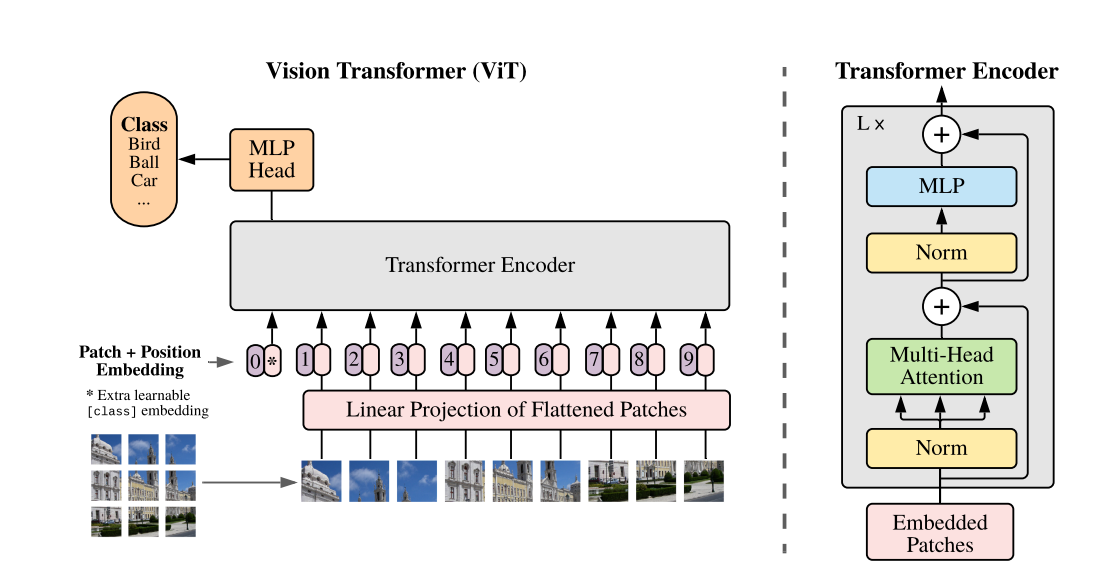
\includegraphics[width=\textwidth]{img/ViT.png}
    \caption{Vision Transformer}\label{fig:vit}
\end{figure}

\begin{figure*}[h]
    \centering
    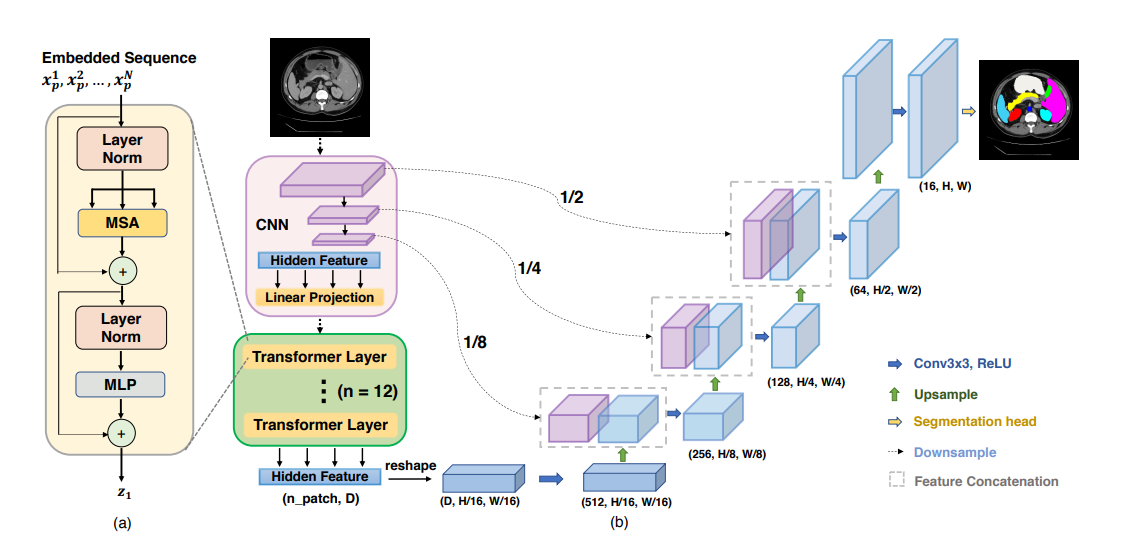
\includegraphics[width=\textwidth]{img/transunet.png}
    \caption{TransUnet Framework}\label{fig:tunet}
\end{figure*}

In the overview of this model, we observe that the image is split into fixed-size patches and is projected linearly after flattening, with an extra positional embedding. After linear projections, these embeddings are fed into a transformer encoder which includes batch normalization, multi-head attention, a multilayer perceptron, and 2 skip-connections. By replacing the word embeddings with flattened image patches, Dosovitskiy \textit{et al.} was able to perform classification on the images.   

\subsection{TransUNet}

\subsubsection{Hybrid Model}
TransUNet is a hybrid network that exploits the local feature encoding characteristics of CNNs and global feature encoding characteristics of the transformers at the same time. As a modification on \cite{dosovitskiy2020image}, TransUNet employs a CNN as a feature extractor to generate a feature map. Then, patch embedding is applied to $1 \times 1$ patches extracted from the CNN feature map instead of the raw images. 

The authors list 2 reasons for following this approach: 1) it allows the utilization of the CNN feature map in the decoding path; 2) it results in better performance when compared to the case the inputs are taken as raw images. 

\begin{equation}
    z_0 = [x_p^1E; x_p^2E; \hdots; x_p^NE] + E_{pos}
    \label{eq:firstinput}
\end{equation}

where $E$ is the patch embedding projection and $E_{pos}$ is the positional embedding. 
Once the input of the first transformer layer is obtained as described in \Cref{eq:firstinput}, the l-th layer output of the transformer can be written as follows: 

\begin{eqnarray}
    {z'}_l &= MSA(LN(z_{l-1})) + z_{l-1} \\
    z_l &= MLP(LN({z'}_l)) + {z'}_l
\end{eqnarray}
\vfill\null\newpage
\subsubsection{Cascaded Upsampler (CUP)}
The decoded feature representation $z_L \in \mathbb{R}^{\frac{HW}{P^2}} \times D$ is reshaped to $\frac{H}{P} \times \frac{W}{P}$. Then, by using 1$\times$1 convolution, the number of channels is reduced to the number of classes. This approach directly applies bilinear upsampling (interpolation) on the coded representation and the resultant tensor is the output result. This na\"ive interpolation approach is called "None" in \cite{chen2021transunet}. Instead of this, the researchers cascade multiple upsampling blocks consisting of 2$\times$ upsampling operator, a $3\times 3$ convolution layer, and ReLU nonlinearity successively. 

\section{Experiments and Results}

\subsection{Performance Metrics} 

The metrics defined in \Cref{eq:DC,eq:HD} are utilized for the evaluation of the performance.

\begin{align}
    Dice \ Coeff.(DSC) &= 2 \times \frac{A \cap B}{A \cup B} \label{eq:DC}\\
    d_H(X,Y) (HD) &= \max \left\{ \sup_{x\in X} d(x,Y),\sup_{b\in B} d(X,y) \right\} \label{eq:HD}
\end{align}

where $A$ and $B$ in \Cref{eq:DC} are target and found segmentation regions, whereas $X$ and $Y$ in \Cref{eq:HD}, the Hausdorff distance, are the segmentation boundaries corresponding to the segmented regions.

When the model predictions show an exact match with labeled regions, both metrics are 1. 

\begin{figure*}[h]
\centering
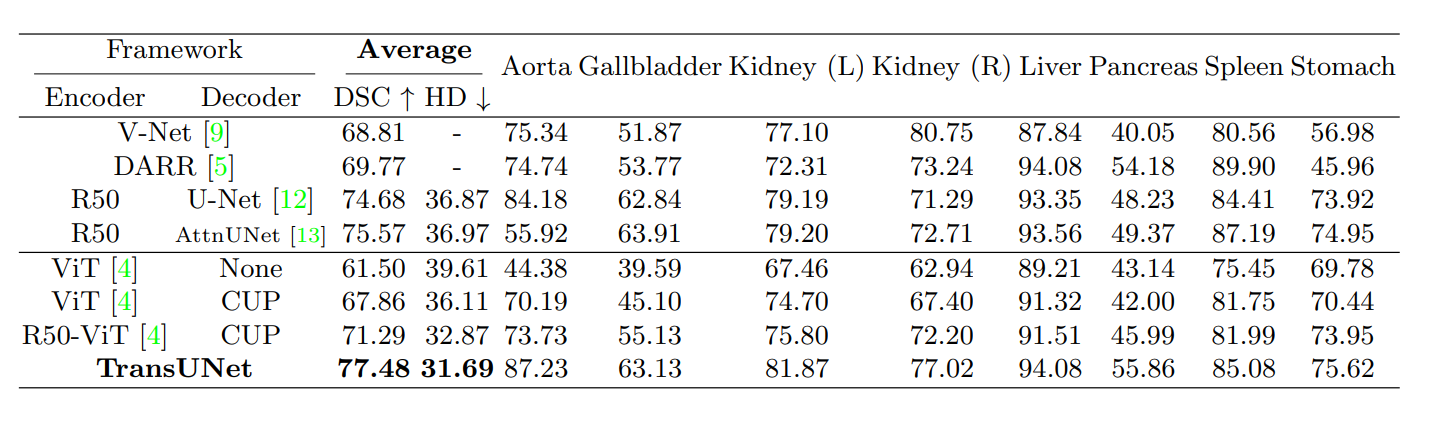
\includegraphics[width=0.8\textwidth]{img/table1.png}
\caption{Comparsion on SYNAPSE dataset}\label{fig:table}
\end{figure*}

\begin{figure*}[h]
\centering
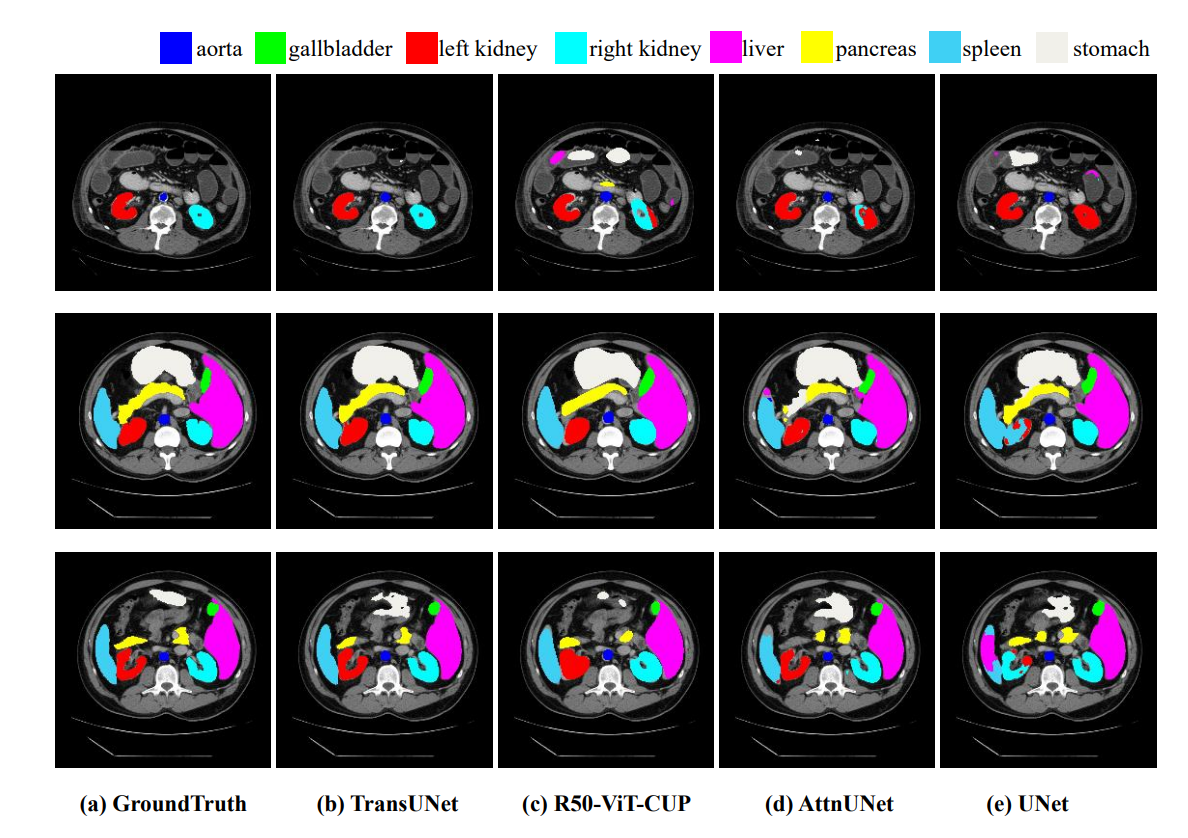
\includegraphics[width=0.8\textwidth]{img/results_qual.png}
\caption{Qualitative results for SYNAPSE dataset}\label{fig:synapseseg}
\end{figure*}

\vfill\null\newpage

\begin{table}[h]
\centering{
\caption{Automated Cardiac Diagnosis Challenge dataset results}\label{tab:acdc}
\begin{tabular}{|c|c|ccc|} \hline
    Framework & Average & RV & Myo & LV \\ \hline
    R50-U-Net & 87.55 & 87.10 & 80.63 & 94.62 \\
    R50-AttnUNet & 86.75 & 87.58 & 79.20 & 93.47\\
    ViT-CUP &81.45 &81.46 &70.71 &92.18\\
    R50-ViT-CUP &87.57 &86.07 &81.88 &94.75\\
    TransUNet &89.71 &88.86 &84.53 &95.73 \\ \hline
\end{tabular}}
\end{table}

\subsection{Original Results \cite{chen2021transunet}}

There are a series of ablation studies to determine the number of skip connections, input resolution, patch size, and sequence length. The latter three are dependent on each other by the relation $P^2L = WH = W^2$, where $P$ is the patch size, $L$ is the sequence length, and $W$ and $H$ are the input image sizes.
PyTorch \cite{paszke2017automatic} deep learning framework is used to train the models.
The models are trained on a single Nvidia RTX2080Ti GPU with the following hyperparameters:
\begin{itemize}
    \item Input size: 224 $\times$ 224
    \item Patch size: 16
    \item Learning rate: 0.01
    \item Momentum 0.9 
    \item Weight decay: 0.0001
    \item Optimizer: Stochastic Gradient Descent
    \item Number of training iterations: 20000
    \item Default batch size: 24
\end{itemize}

\begin{figure*}[h]
\centering
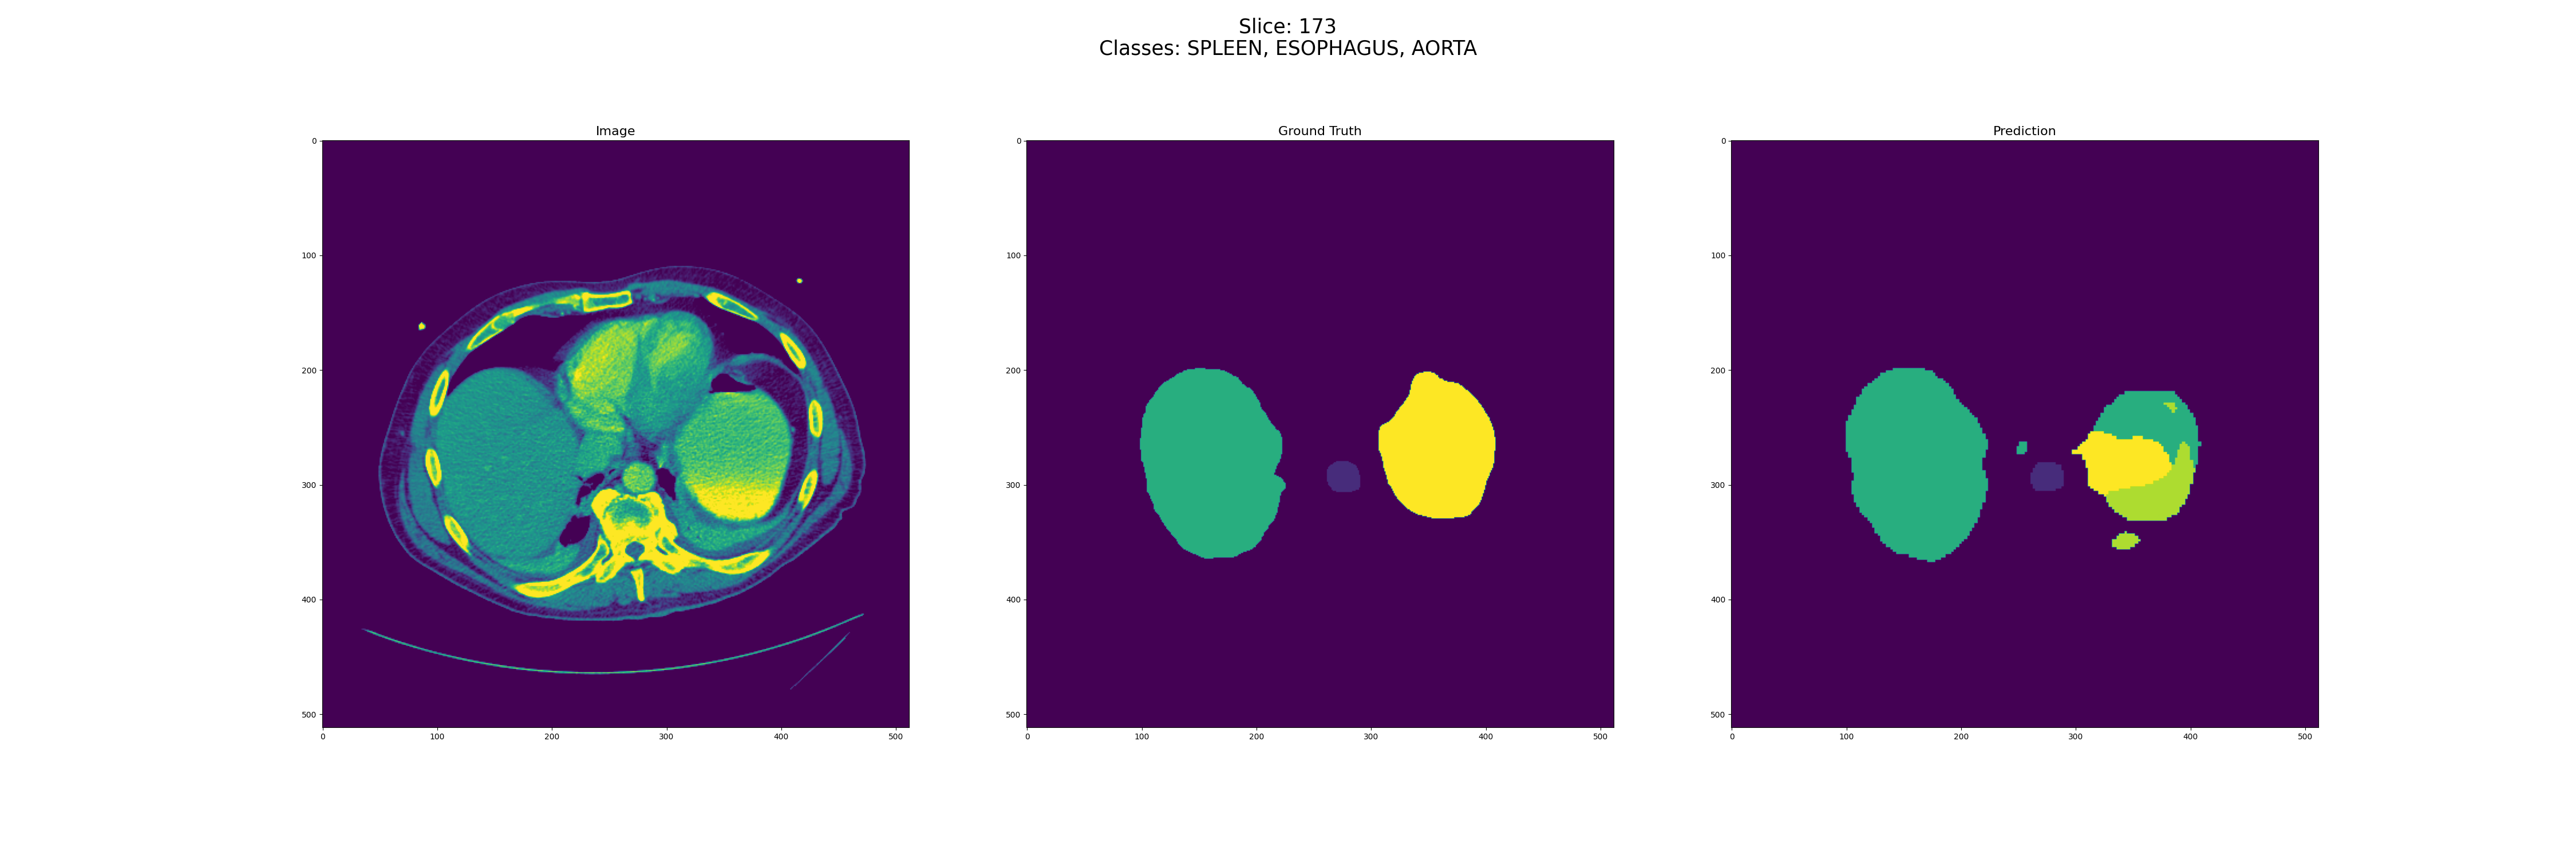
\includegraphics[width=\textwidth]{img/slice_173.png}
\caption{False positive predictions in Slice 173 in concatenated data}\label{fig:slice1}
\end{figure*}
\begin{figure*}[h]
\centering
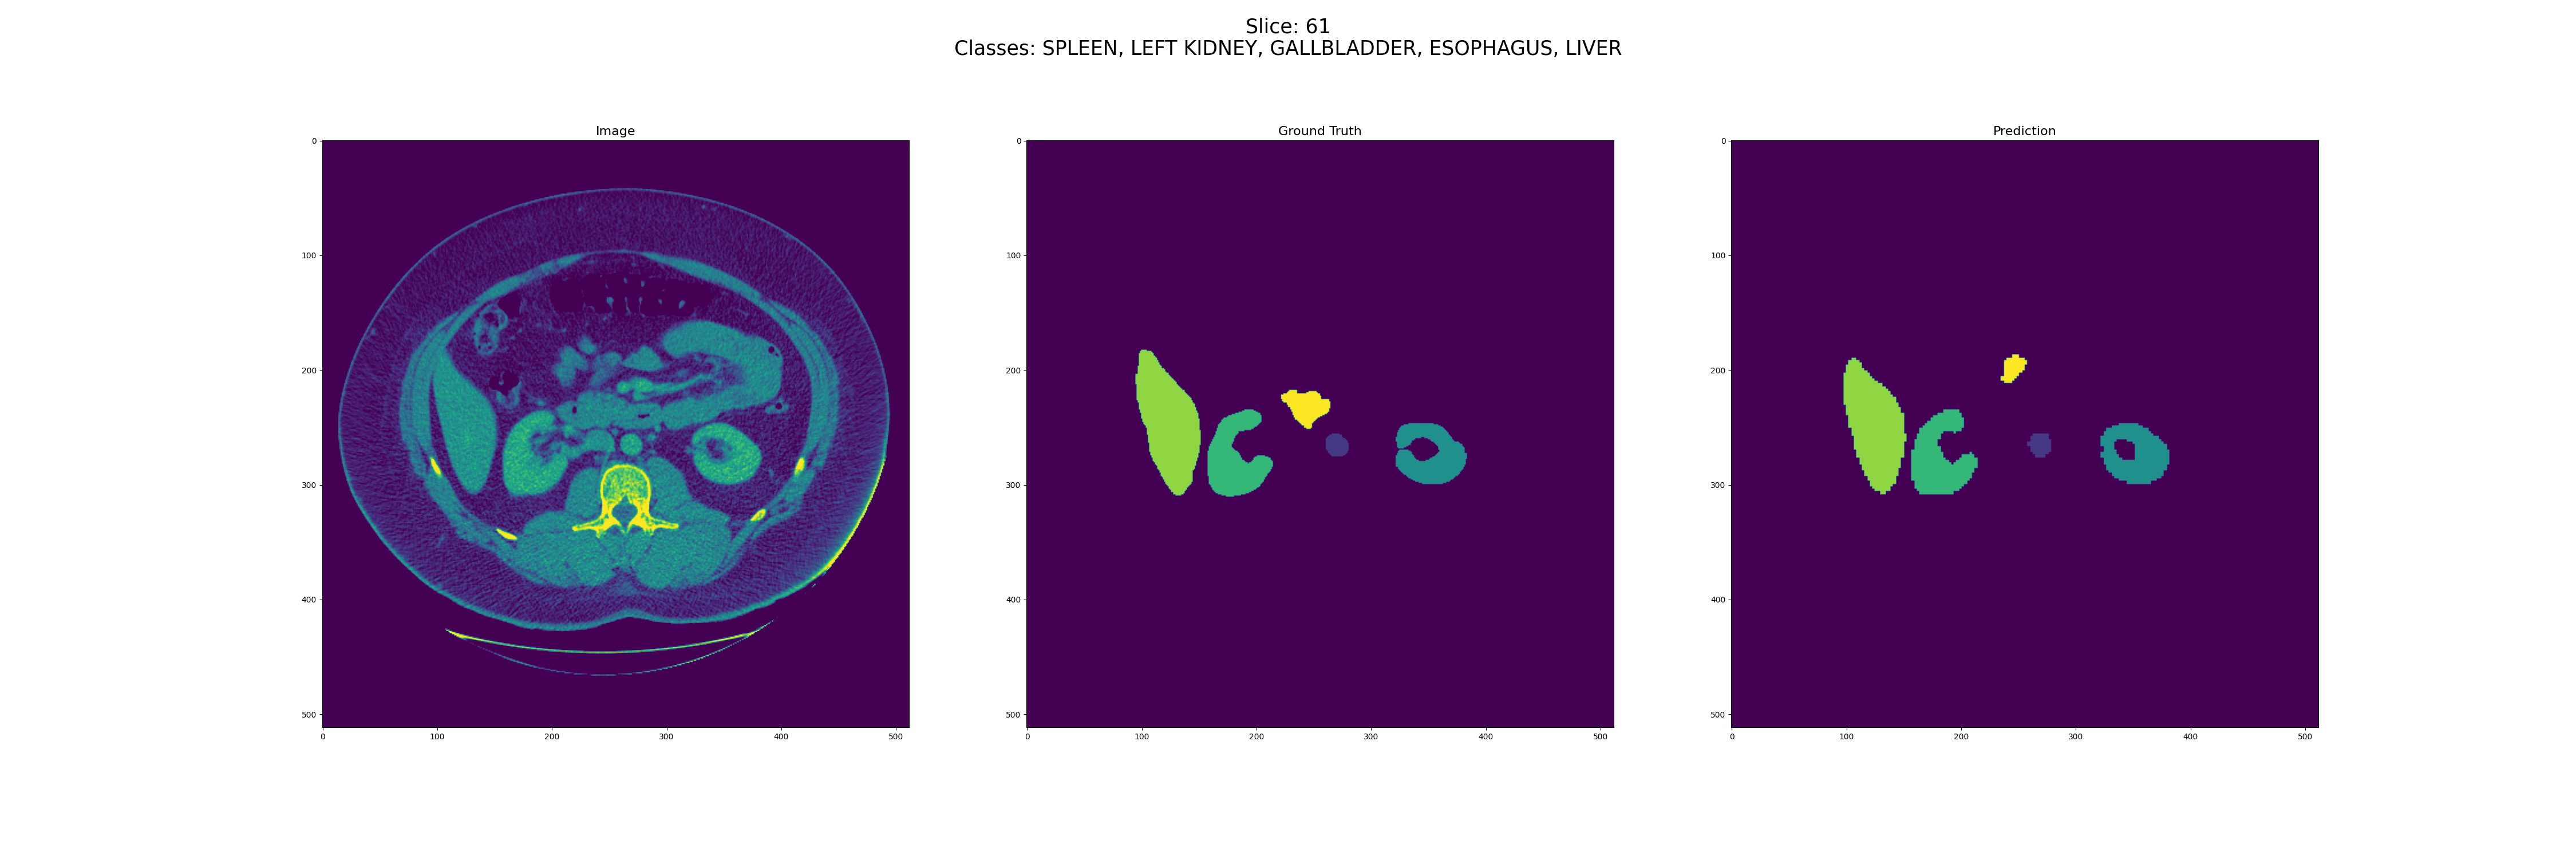
\includegraphics[width=\textwidth]{img/slice_61.png}
\caption{Predictions in Slice 61 in concatenated data}\label{fig:slice2}
\end{figure*}

The TransUNet model that is used to produce these results is what is referred to as \textbf{base} model in the ablation results. To train the proposed network, Chen \textit{et al.} used 30 abdominal CT scans in the MICCAI 2015 Multi-Atlas Abdomen Labelling Challenge, adding up to 3779 axial contrast-enhanced images from the SYNAPSE dataset and ACDC dataset. The experiments are done with different encoder and decoder architectures and the average DSC in percentage and Hausdorff distance in millimeters for eight abdominal organs with a random split 18 training and 12 validation cases are reported. Looking at \Cref{fig:table}, we see that TransUNet outperforms the best predecessor by 2.8\% in terms of average DSC and it reduced the HD by approximately 3\% when compared with the best predecessor. It is possible to investigate that the proposed method's performance is the best for 4 organs presented in \Cref{fig:table}. In \Cref{tab:acdc}, we observe that for both metrics, TransUNet outperformed the others for segmentation classes Left Ventricle, Myocardium, and Right Ventricle.

\subsection{Replicated Results}

\begin{figure}[h]
\centering
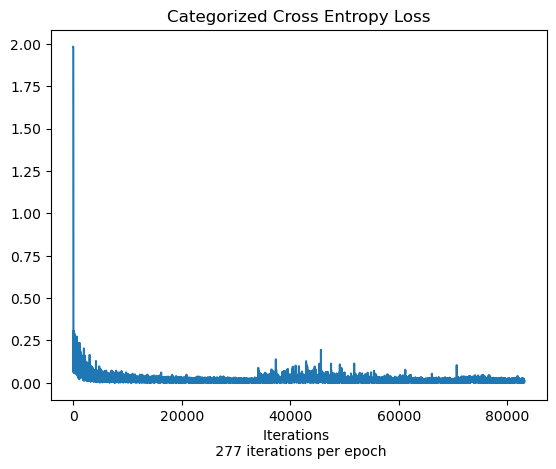
\includegraphics[width=0.8\textwidth]{img/celoss.png}
\caption{Cross entropy loss during training}\label{fig:celoss}
\end{figure}

\subsubsection{Training}
The models are trained on a single NVIDIA GeForce GTX 1660 Ti on TU116-A GPU
with the following hyperparameters:
\begin{itemize}
    \item Input size: 224 $\times$ 224
    \item Patch size: 16
    \item Learning rate: 0.01
    \item Momentum 0.9 
    \item Weight decay: 0.0001
    \item Optimizer: Stochastic Gradient Descent
    \item Number of training epochs: 150
    \item Batch size: 8
\end{itemize} 
For training, argparser that is provided in the original repository is utilized as explained the documentation. The batch size is updated due to the limited GPU memory size. With the given configuration above, the training took 18 hours with 150 epochs on 83 scans with 1009 slices that were provided as averaged training images. 

\subsubsection{Inference}
On inference time, 12 different test cases were evaluated. The inference took approximately 2 minutes per case on average. DSC and HD are calculated between the ground truth and the model outputs slice-by-slice and the mean of the metrics along the slice dimension is calculated for each test case. Then, mean$\pm$std DC metric is calculated along with the median(IQR) HD metric are calculated for each test case:

\begin{itemize}
    \item DSC: 0.7810 $\pm$ 0.0841
    \item HD: 10.9264 (35.5377)
\end{itemize}

The network produces only 8 organs' individual results. For the inference whose results given above, the corresponding evaluations for individual organs are presented in \Cref{tab:organs}. Although most of the predictions match with corresponding ground truth labelings as shown in \Cref{fig:slice2}, there were some cases where some false positive detections are identified. This may be due to the undertrained model due to the given limited time and computational resources. Although we expect the model to find 3 different classes in \Cref{fig:slice1}, there were 5 different classes predicted in the inference time. 

\begin{table}[h]
\caption{\label{tab:organs}Segmentation performance on individual organs utilized in the study}
\centering{
\begin{tabular}{|c|c|c|} \hline
    \diagbox{Organ}{Metric} & DSC & \makecell{HD\\(mm)} \\ \hline
    Aorta & 0.86 & 13.85\\ \hline
    Gallbladder & 0.64 & 18.74\\ \hline
    Spleen & 0.83 & 41.36\\ \hline
    Left Kidney & 0.79 & 33.65\\ \hline
    Right Kidney & 0.92 & 37.61\\ \hline
    Liver & 0.61 & 15.07\\ \hline
    Pancreas & 0.86 & 45.46\\ \hline
    Spleen & 0.76 & 21.03\\ \hline
\end{tabular}}
\end{table}

\section{Conclusion}

In this project report, the study \textit{TransUNet: Transformers Make Strong Encoders for Medical Image Segmentation} is analyzed and some of the results were replicated in different training and testing configurations. The results are satisfying given the model's size and predictions, even when compared with the state-of-the-art. Although detailed ablation studies for different hyperparameters are already conducted, the inference can be improved by training the model on a dataset that has more diverse distributions. 

\vfill\null\newpage
\printbibliography{}
\end{document}